\documentclass[]{llncs}
\usepackage{graphicx}

%\documentclass{article}
\usepackage{mathtools}
\usepackage{times}  % DO NOT CHANGE THIS
\usepackage{helvet} % DO NOT CHANGE THIS
\usepackage{courier}  % DO NOT CHANGE THIS
\usepackage[hyphens]{url}  % DO NOT CHANGE THIS
\usepackage{arydshln}
\usepackage{mathptmx}
\usepackage{amsmath}
\usepackage{bm}
\usepackage[english]{babel}
\usepackage[utf8]{inputenc}
\usepackage{algorithm}
\usepackage{epstopdf}
\usepackage{booktabs}
\usepackage{multirow}
\usepackage{siunitx}
\usepackage{rotating}
\usepackage{hyperref}
%\usepackage[algo2e]{algorithm2e}
%\usepackage{arevmath}     % For math symbols
\usepackage[noend]{algpseudocode}
\urlstyle{rm} % DO NOT CHANGE THIS
\def\UrlFont{\rm}  % DO NOT CHANGE T
% Used for displaying a sample figure. If possible, figure files should
% be included in EPS format.
%
% If you use the hyperref package, please uncomment the following line
% to display URLs in blue roman font according to Springer's eBook style:
% \renewcommand\UrlFont{\color{blue}\rmfamily}

\pagestyle{plain}
\setcounter{page}{1}
\pagenumbering{arabic}

\DeclareMathOperator*{\argmax}{argmax} 

\begin{document}

\title{Mathematics for Beliefs Strategy Approach}

\author{Frances Cameron-Muller, Supervisor: Dr. Julian Garcia}

\institute{Monash University}

\maketitle    

\section{Introduction}
In the individual learning model, every agent has an belief about how both types of agents will play. These beliefs represent the probability of ingroup/outgroup individuals cooperating. 

\section{Definitions}

\subsection{Bayesian Games} 
A Bayesian game consists of: \\
A set of players: $I$\\
A set of actions (pure strategies) for each player i: $S_i$\\
A set of types for each player i: $\theta_i  \in \Theta_i $ \\
A payoff function for each player i: $u_i(\,s_1, . . . ,s_I, \theta_1, . . . , \theta_I)\,$\\
A (joint) probability distribution $p(\,\theta_1, . . . , \theta_I)\,$ over types 

\subsection{Specifics for this model}
Player i's belief about type $\theta$ :  $b_{i,\theta}$ \\ 
\[
   \text{Payoff Matrix} = \begin{pmatrix} 
   R & S  \\
   T & P  
   \end{pmatrix} 
\]
\\
Payoff Threshold: $H = \frac{S-P}{T-P-R+S}$ \\
Number of agents: $n$ \\ 
Set of actions (pure strategies) for each player i: $S_i = \{0 (\,Cooperate)\, ,1 (\,Defect)\,\}$\\
Set of types for each player i: $ \Theta_i = \{0,1\}$ \\
Payoff function for each player i: $u_i(\,s_1, . . . ,s_I, \theta_1, . . . , \theta_I)\,$\\
\\
Payoff function of player i with strategy $s_i \in S_i$ and type $\theta_i$ against an opponent with strategy $s_{-i}$ and type $\theta_{-i}$
\[
   u_i(\,s_i, s_{-i}(\,\theta_{-i})\,,  \theta_i, \theta_{-i})\, =  \begin{cases}
        R & if\ s_i = 0 \cap s_{-i} = 0 \\
        S & if\ s_i = 0 \cap s_{-i} = 1 \\
        T & if\ s_i = 1 \cap s_{-i} = 0 \\
        P & if\ s_i = 1 \cap s_{-i} = 1 \\
    \end{cases}
\]
or equivalently 
\[
   u_i(\,s_i, s_{-i}(\,\theta_{-i})\,,  \theta_i, \theta_{-i})\, =  \begin{cases}
        R & if\ b_{i,\theta_{-i}} \geq H \cap b_{-i,\theta_{i}}  \geq H \\
        S & if\ b_{i,\theta_{-i}}  \geq H \cap b_{-i,\theta_{i}} < H \\
        T & if\ b_{i,\theta_{-i}}  < H \cap b_{-i,\theta_{i}} \geq H \\
        P & if\ b_{i,\theta_{-i}} < H \cap b_{-i,\theta_{i}} < H \\
    \end{cases}
\]


\section{Expected Payoff}

Using Bayes rule, the expected payoffs of player i of type $\theta_i$ with a strategy $s_i'$ is 
\[
U(\,s_i', s_{-i}(\, . )\,, \theta_i)\, = \sum\limits_{\theta_{-i}} p(\, \theta_{-i} \mid \theta_i)\, u_i(\,s_i', s_{-i}(\, \theta_{-i} )\,, \theta_i, \theta_{-i})\,
\]
\\
The strategy profile s(.) is a (pure strategy) Bayesian Nash equilibrium if for all $i \in I$ and for all $\theta_i \in \Theta_i$, we have that 
\[
s_i(\,\theta_i)\, \in \argmax\limits_{s_i' \in S_i} \sum\limits_{\theta_{-i}} p(\, \theta_{-i} \mid \theta_i)\, u_i(\,s_i', s_{-i}(\, \theta_{-i} )\,, \theta_i, \theta_{-i})\,
\]
\\
The expression for expected payoff represents the sum of the conditional probabilities that an opponent is type $\theta_{-i}$ given the agent is type $\theta_i$ multiplied with the payoff agent i would receive against an agent of this type.\\
Unfortunately, we have incomplete information in our model and agent i doesn't know the beliefs or behaviour of the other players. Therefore we extend the model so that agent i has a prior guess of the how the other agents will play against them.\\
Agent's priors of how agents of a certain type will behave is represented by a Normal distribution. It is specified by a mean that represents the probability they expect agents of that type will cooperate and a variance that describes their uncertainty in their prior guess. \\

\subsection{Example}

Consider a model with, 3 agents (n = 3) of types $\theta = (\, \theta_1, \theta_2, \theta_3)\, = (\, 0,0,1)\,.$\\
The proportion of agents of type 0, $p = \frac{2}{3}$.\\
\[
   \text{Payoff Matrix} = \begin{pmatrix} 
   6 & 1  \\
   3 & 2  
   \end{pmatrix} 
\]
Agent 1 has prior guesses of $N(\,0.9,1)\,$ and $N(\,0.1,1)\,$ for types 0 and 1, respectively. \\
\\
The expected payoff of player 1 playing a strategy of $s_1' = 0$
\[ 
U(\,s_1' = 0,  s_{-1}(\, . )\,, \theta_1 = 0)\, = \sum\limits_{\theta_{-i}} p(\, \theta_{-i} \mid \theta_i)\, u_i(\,s_i', s_{-i}(\, \theta{-i} )\,, \theta_i, \theta_{-i})\, 
\]
\[
= p(\, \theta_{2} \mid \theta_1)\, u_1(\,s_1' = 0, s_{2}(\, \theta_{2} )\,, \theta_1, \theta_{2})\, +  p(\, \theta_{3} \mid \theta_1)\, u_1(\,s_1' = 0, s_{3}(\, \theta{3} )\,, \theta_1, \theta_{3})\,
\] 
\[
= p(\, 0 \mid 0)\,  \times R + p(\, 1 \mid 0)\,  \times S
\]
\[
= \frac{1}{2} \times 6 + \frac{1}{2} \times 1 = 3.5
\]
\\
The expected payoff for player 1 with a strategy of 1 is 
\[ 
U(\,s_1' = 1,  s_{-1}(\, . )\,, \theta_1 = 0)\, = \sum\limits_{\theta_{-i}} p(\, \theta_{-i} \mid \theta_i)\, u_i(\,s_i', s_{-i}(\, \theta{-i} )\,, \theta_i, \theta_{-i})\, 
\]
\[
= p(\, \theta_{2} \mid \theta_1)\, u_1(\,s_1' = 1, s_{2}(\, \theta_{2} )\,, \theta_1, \theta_{2})\, +  p(\, \theta_{3} \mid \theta_1)\, u_1(\,s_1' = 1, s_{3}(\, \theta{3} )\,, \theta_1, \theta_{3})\,
\]
\[
= p(\, 0 \mid 0)\,  \times T + p(\, 1 \mid 0)\,  \times P
\]
\[
= \frac{1}{2} \times 3 + \frac{1}{2} \times 2 = 2.5
\]
\\
Therefore, the Bayesian Nash equilibrium given these conditions is 
\[
s_i(\,\theta_i)\, \in \argmax\limits_{s_i' \in S_i} \sum\limits_{\theta_{-i}} p(\, \theta_{-i} \mid \theta_i)\, u_i(\,s_i', s_{-i}(\, \theta{-i} )\,, \theta_i, \theta_{-i})\,
\]
\[
s_1(\,0)\, = 0
\]
The Bayesian Nash Equilibrium solution for agent 1 in this model given the prior distribution is cooperating. 

\subsection{Extensions}
We can vary parameters such as prior beliefs, payoff matrix and proportion of each type to see the effect on the expected payoffs and optimal strategies of the agents. 

\section{Experiments}
\begin{figure}
\centering
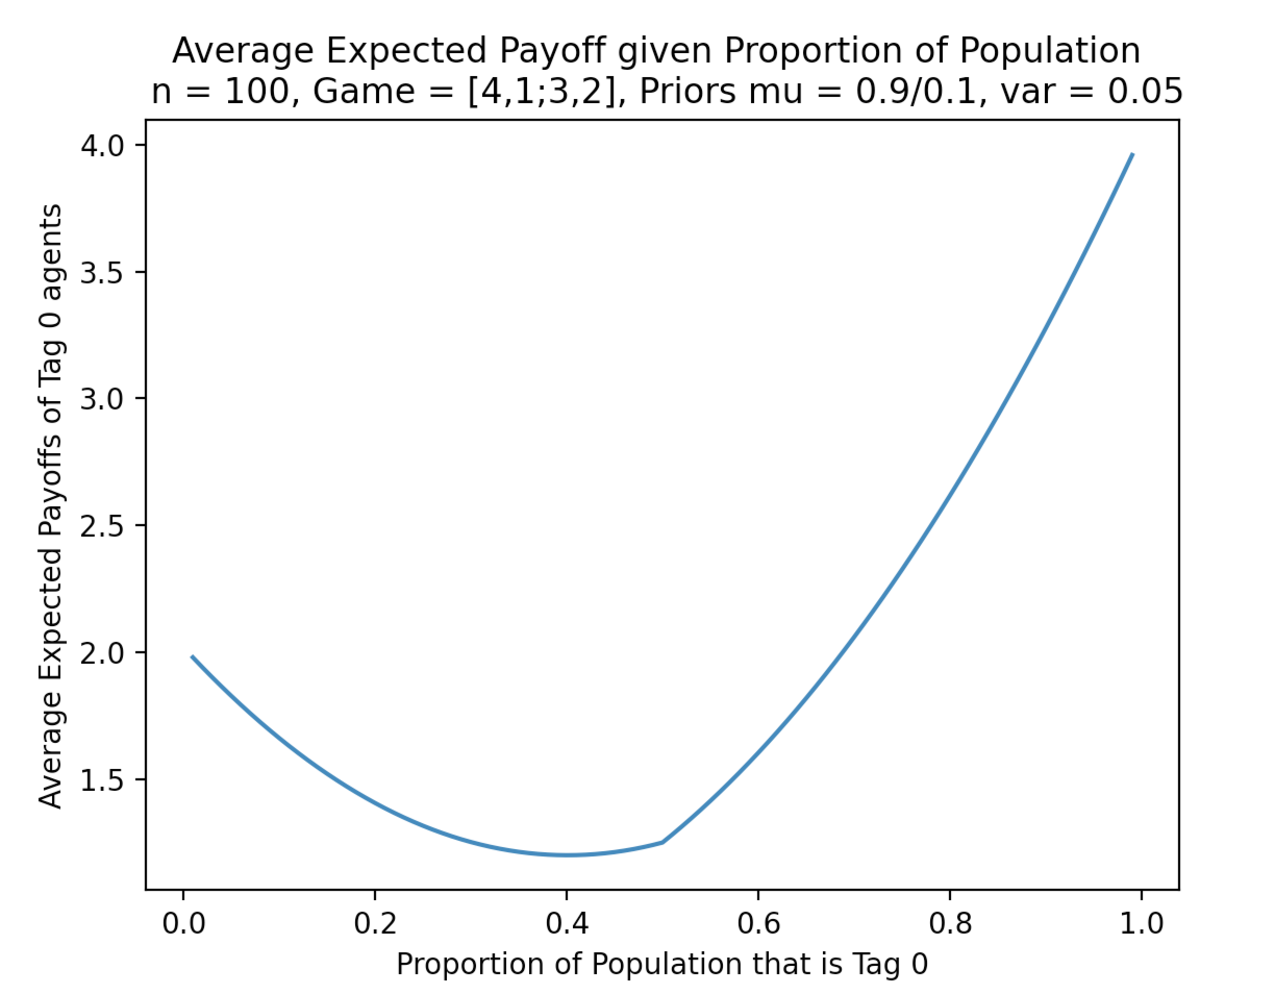
\includegraphics[width=12cm]{images/p_experiment}
\end{figure}

\begin{figure}
\centering
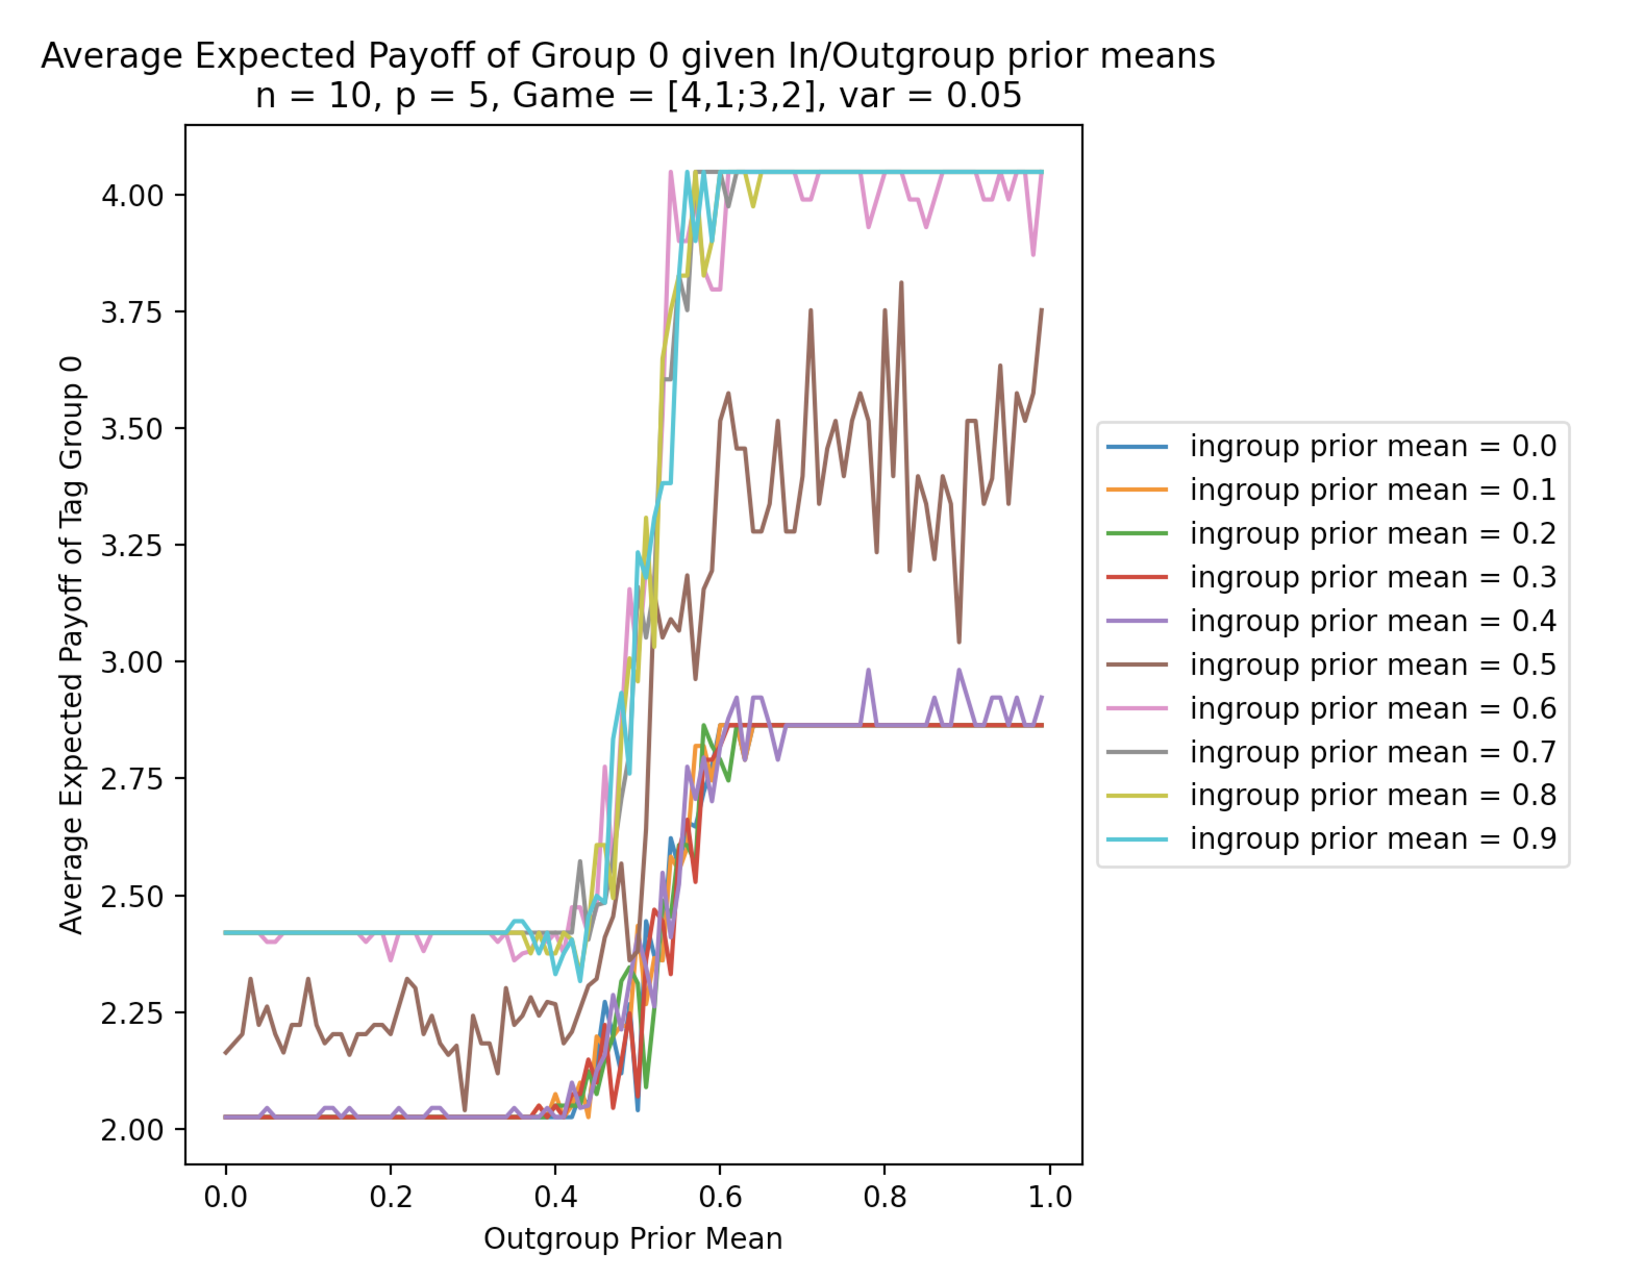
\includegraphics[width=12cm]{images/prior_experiment}
\end{figure}


\end{document}
